%==============================================================================
% tento soubor pouzijte jako zaklad
% this file should be used as a base for the thesis
% (c) 2008 Michal Bidlo
% E-mail: bidlom AT fit vutbr cz
% Šablonu upravil / template edited by: Ing. Jaroslav Dytrych, dytrych@fit.vutbr.cz
%==============================================================================
% kodovaní: UTF-8 (zmena prikazem iconv, recode nebo cstocs)
% encoding: UTF-8 (you can change it by command iconv, recode or cstocs)
%------------------------------------------------------------------------------
% zpracování / processing: make, make pdf, make clean
%==============================================================================
% Soubory, které je nutné upravit: / Files which have to be edited:
%   projekt-20-literatura-bibliography.bib - literatura / bibliography
%   projekt-01-kapitoly-chapters.tex - obsah práce / the thesis content
%   projekt-30-prilohy-appendices.tex - přílohy / appendices
%==============================================================================
\documentclass[zadani]{fitthesis} % bez zadání - pro začátek práce, aby nebyl problém s překladem
%\documentclass[english]{fitthesis} % without assignment - for the work start to avoid compilation problem
%\documentclass[zadani]{fitthesis} % odevzdani do wisu - odkazy jsou barevné
%\documentclass[english,zadani]{fitthesis} % for submission to the IS FIT - links are color
%\documentclass[zadani,print]{fitthesis} % pro tisk - odkazy jsou černé
%\documentclass[english,zadani,print]{fitthesis} % for the print - links are black
% * Je-li prace psana v anglickem jazyce, je zapotrebi u tridy pouzit 
%   parametr english nasledovne:
%   If thesis is written in english, it is necessary to use 
%   parameter english as follows:
%      \documentclass[english]{fitthesis}
% * Je-li prace psana ve slovenskem jazyce, je zapotrebi u tridy pouzit 
%   parametr slovak nasledovne:
%      \documentclass[slovak]{fitthesis}

% Základní balíčky jsou dole v souboru šablony fitthesis.cls
% Basic packages are at the bottom of template file fitthesis.cls
%zde muzeme vlozit vlastni balicky / you can place own packages here

%---rm---------------
\renewcommand{\rmdefault}{lmr}%zavede Latin Modern Roman jako rm / set Latin Modern Roman as rm
%---sf---------------
\renewcommand{\sfdefault}{qhv}%zavede TeX Gyre Heros jako sf
%---tt------------
\renewcommand{\ttdefault}{lmtt}% zavede Latin Modern tt jako tt

% vypne funkci šablony, která automaticky nahrazuje uvozovky,
% aby nebyly prováděny nevhodné náhrady v popisech API apod.
% disables function of the template which replaces quotation marks
% to avoid unnecessary replacements in the API descriptions etc.
\csdoublequotesoff

% =======================================================================
% balíček "hyperref" vytváří klikací odkazy v pdf, pokud tedy použijeme pdflatex
% problém je, že balíček hyperref musí být uveden jako poslední, takže nemůže
% být v šabloně
% "hyperref" package create clickable links in pdf if you are using pdflatex.
% Problem is that this package have to be introduced as the last one so it 
% can not be placed in the template file.
\ifWis
\ifx\pdfoutput\undefined % nejedeme pod pdflatexem / we are not using pdflatex
\else
  \usepackage{color}
  \usepackage[unicode,colorlinks,hyperindex,plainpages=false,pdftex]{hyperref}
  \definecolor{links}{rgb}{0.4,0.5,0}
  \definecolor{anchors}{rgb}{1,0,0}
  \def\AnchorColor{anchors}
  \def\LinkColor{links}
  \def\pdfBorderAttrs{/Border [0 0 0] }  % bez okrajů kolem odkazů / without margins around links
  \pdfcompresslevel=9
\fi
\else % pro tisk budou odkazy, na které se dá klikat, černé / for the print clickable links will be black
\ifx\pdfoutput\undefined % nejedeme pod pdflatexem / we are not using pdflatex
\else
  \usepackage{color}
  \usepackage[unicode,colorlinks,hyperindex,plainpages=false,pdftex,urlcolor=black,linkcolor=black,citecolor=black]{hyperref}
  \definecolor{links}{rgb}{0,0,0}
  \definecolor{anchors}{rgb}{0,0,0}
  \def\AnchorColor{anchors}
  \def\LinkColor{links}
  \def\pdfBorderAttrs{/Border [0 0 0] } % bez okrajů kolem odkazů / without margins around links
  \pdfcompresslevel=9
\fi
\fi
% Řešení problému, kdy klikací odkazy na obrázky vedou za obrázek
% This solves the problems with links which leads after the picture
\usepackage[all]{hypcap}
\usepackage{tikz}
\usepackage{gensymb}
 \usepackage{dirtree}
 
\usetikzlibrary{shadows}
% znaky klavesnice
\newcommand*\keystroke[1]{%
	\tikz[baseline=(key.base)]
	\node[%
	draw,
	fill=white,
	drop shadow={shadow xshift=0.25ex,shadow yshift=-0.25ex,fill=black,opacity=0.75},
	rectangle,
	rounded corners=2pt,
	inner sep=2pt,
	line width=0.5pt,
	font=\scriptsize\sffamily
	](key) {#1\strut}
	;
}


% Informace o práci/projektu / Information about the thesis
%---------------------------------------------------------------------------
\projectinfo{
  %Prace / Thesis
  project=BP,            %typ prace BP/SP/DP/DR  / thesis type (SP = term project)
  year=2017,             %rok odevzdání / year of submission
  date=\today,           %datum odevzdani / submission date
  %Nazev prace / thesis title
  title.cs={Webový prohlížeč panoramatických snímků},  %nazev prace v cestine ci slovenstine (dle zadani) / thesis title in czech language (according to assignment)
  title.en={Web-based Panorama image viewer}, %nazev prace v anglictine / thesis title in english
  %Autor / Author
  author={Tomáš Slunský},   %cele jmeno a prijmeni autora / full name and surname of the author
  author.name={Tomáš},   %jmeno autora (pro citaci) / author name (for reference) 
  author.surname={Slunský},   %prijmeni autora (pro citaci) / author surname (for reference) 
  %author.title.p=Bc., %titul pred jmenem (nepovinne) / title before the name (optional)
  %author.title.a=PhD, %titul za jmenem (nepovinne) / title after the name (optional)
  %Ustav / Department
  department=UPGM, % doplnte prislusnou zkratku dle ustavu na zadani: UPSY/UIFS/UITS/UPGM
  %                  fill in appropriate abbreviation of the department according to assignment: UPSY/UIFS/UITS/UPGM
  %Skolitel / supervisor
  supervisor=Martin Čadík, %cele jmeno a prijmeni skolitele / full name and surname of the supervisor
  supervisor.name={Martin},   %jmeno skolitele (pro citaci) / supervisor name (for reference) 
  supervisor.surname={Čadík},   %prijmeni skolitele (pro citaci) / supervisor surname (for reference) 
  supervisor.title.p=Doc. Ing.,   %titul pred jmenem (nepovinne) / title before the name (optional)
  supervisor.title.a={Ph.D.},    %titul za jmenem (nepovinne) / title after the name (optional)
  %Klicova slova, abstrakty, prohlaseni a podekovani je mozne definovat 
  %bud pomoci nasledujicich parametru nebo pomoci vyhrazenych maker (viz dale)
  %Keywords, abstracts, declaration and acknowledgement can be defined by following 
  %parameters or using dedicated macros (see below)
  %===========================================================================
  %Klicova slova / keywords
  %keywords.cs={Klíčová slova v českém jazyce.}, %klicova slova v ceskem ci slovenskem jazyce
  %                                              keywords in czech or slovak language
  %keywords.en={Klíčová slova v anglickém jazyce.}, %klicova slova v anglickem jazyce / keywords in english
  %Abstract
  %abstract.cs={Výtah (abstrakt) práce v českém jazyce.}, % abstrakt v ceskem ci slovenskem jazyce
  %                                                         abstract in czech or slovak language
  %abstract.en={Výtah (abstrakt) práce v anglickém jazyce.}, % abstrakt v anglickem jazyce / abstract in english
  %Prohlaseni / Declaration
  %declaration={Prohlašuji, že jsem tuto bakalářskou práci vypracoval samostatně pod vedením pana ...},
  %Podekovani (nepovinne) / Acknowledgement (optional)
  %acknowledgment={Zde je možné uvést poděkování vedoucímu práce a těm, kteří poskytli odbornou pomoc.} % nepovinne
  %acknowledgment={Here it is possible to express thanks to the supervisor and to the people which provided professional help.} % optional
}

%Abstrakt (cesky, slovensky ci anglicky) / Abstract (in czech, slovak or english)
\abstract[cs]{Účelem práce je navrhnout a realizovat prohlížeč sférických videí a panoramatických fotek. Důraz je kladen na zpracování videí v režimu rybího oka. Mezi další aspekty práce patří vylepšení prohlížeče  grafické prvky, jako je kompas, nebo informace i zorném úhlu pozorovatele. }

\abstract[en]{The purpose of this bachelors thesis is the implementation of panoramic viewer of videos and images. Thesis is focussing   on processing videos, which are in fisheye mode. Between other aspects of this thesis belongs for instance the improvemenst of panoramic viewer with compass, or with  informations about viewers angle.}

%Klicova slova (cesky, slovensky ci anglicky) / Keywords (in czech, slovak or english)
\keywords[cs]{WebGL, HTML5, javascript, panoráma, sférické video, prohlížeč}
\keywords[en]{WebGL, HTML5, javascript, panorama, spherical video, viewer}

%Prohlaseni (u anglicky psane prace anglicky, u slovensky psane prace slovensky)
%Declaration (for thesis in english should be in english)
\declaration{Prohlašuji, že jsem tuto bakalářskou práci vypracoval samostatně pod vedením pana X...
Další informace mi poskytli...
Uvedl jsem všechny literární prameny a publikace, ze kterých jsem čerpal.}

% \declaration{Hereby I declare that this bachelor's thesis was prepared as an original author’s work under the supervision of Mr. X
% The supplementary information was provided by Mr. Y
% All the relevant information sources, which were used during preparation of this thesis, are properly cited and included in the list of references.}

%Podekovani (nepovinne, nejlepe v jazyce prace) / Acknowledgement (optional, ideally in the language of the thesis)
\acknowledgment{Rád bych poděkoval Martinu Čadíkovi za jeho cenné rady, vedení při tvorbě bakalářské práce a jeho celkový přístup. Dále bych rád poděkoval své rodině a blízkým za jejich trpělivost, toleranci a pochopení.}
%\acknowledgment{Here it is possible to express thanks to the supervisor and to the people which provided professional help
%(external submitter, consultant, etc.).}

% řeší první/poslední řádek odstavce na předchozí/následující stránce
% solves first/last row of the paragraph on the previous/next page
\clubpenalty=10000
\widowpenalty=10000

\begin{document}
  % v pripade zmeny souradnic v implementaci je potreba definvoat souradnice centralni
  % aby se nemusely menit na kazde strance zvlast
	\newcommand{\axisX}{x}
	\newcommand{\axisY}{y}
	\newcommand{\axisZ}{z}
	\newcommand{\createSphereGeometry}{createSphereGeometry()}	
	\newcommand{\initProgram}{initProgram()}
	\newcommand{\setupProgram}{setupProgram()}
	\newcommand{\render}{render()}
	\newcommand{\main}{main()}
	\newcommand{\createVideoControlls}{createVideoControlls()}
	\newcommand{\createCompass}{createCompass()}
	\newcommand{\createCompassFull}{createCompass(width, height, position\_x, position\_y, north\_position, angle)	}
	\newcommand{\updateTexture}{updateTexture()}
	\newcommand{\createFieldVision}{createFieldVision()}
	
  % Vysazeni titulnich stran / Typesetting of the title pages
  % ----------------------------------------------
  \maketitle
  % Obsah
  % ----------------------------------------------
  \tableofcontents
  
  % Seznam obrazku a tabulek (pokud prace obsahuje velke mnozstvi obrazku, tak se to hodi)
  % List of figures and list of tables (if the thesis contains a lot of pictures, it is good)
\ifczech
  \renewcommand\listfigurename{Seznam obrázků}
\fi
\ifslovak
  \renewcommand\listfigurename{Zoznam obrázkov}
\fi

   \listoffigures
\ifczech
  \renewcommand\listtablename{Seznam tabulek}
\fi
\ifslovak
  \renewcommand\listtablename{Zoznam tabuliek}
\fi

  % \listoftables 

  % vynechani stranky v oboustrannem rezimu
  % Skip the page in the two-sided mode
  \iftwoside
    \cleardoublepage
  \fi

  % Text prace / Thesis text
  % ----------------------------------------------
  %=========================================================================
% (c) Michal Bidlo, Bohuslav Křena, 2008
\setcounter{secnumdepth}{4} % cislovani nadpisu do hloubky



\chapter{Úvod}
\label{chapter:1}

V současné době se technologie ve všech odvětvích stále posouvá a~není tomu jinak ani u~prohlížení fotek a~videí. V současné době i~takto nahrané informace pomocí digitálních zařízení je trend dále posouvat a~zvyšovat tak zážitek ze zaznamenané události. Díky tomuto trendu si už nevystačíme s ``klasickými''  přehrávači, popř. prohlížeči videí, nebo fotografií. Díky sférickým 360 stupňovým kamerám, je dnes možné zaznamenat video o~srovnatelné velikosti jako u dnes běžného telefonu, ale s~mnohem větším objemem informací, které se ale nedají srozumitelně přehrát v~klasických přehrávačích. Ruku v ruce se sdílením takových dát, je velice výhodné takový prohlížeč nabídnout jako webovou verzi, aby i~jiní uživatelé mohli svá takto natočená videa přehrávat popř. sdílet. Důkazem toho je rozmach multimediálního obsahu na internetu, kdy samotný jazyk HTML pro prezentaci webových stránek dříve nenabízel přímou podporu videí, což se změnilo příchodem nové verze HTML5. Některé portály jako např. Youtube již dnes začíná nasazovat do svého prohlížení videí jeho rozšířené sférické verze, což tedy potvrzuje tento trend. Tato práce má za cíl takové prohlížení posunout ještě dál.


Následující práce se věnuje implementaci webového prohlížeče panoramatických snímku a videí v různých módech, ve kterých je video interpretováno. Cílem je tedy navrhnout a zrealizovat řešení, aby uživatel po natočení videa dále nepotřeboval k přehrání např. sférického videa v režimu rybího oka specifický program, který by video musel nejprve překonvertovat. To stejné se týká i~panoramatických snímku a~videí v equirectangulárním zobrazení.  


Další inovací v prohlížení videí je přidání některých dat, které v běžném prohlížení nejsou k dispozici. Např. informace o světových stranách ve vztahu k obrázku, či videu popřípadě údaje o velikosti zorného pole v daném kontextu prohlížení až po dodatečná metadata v~panoramatických obrázcích, které jsou vhodné např. k~tomu, aby autor obrázku mohl popsat jeho zajímavé částí popřípadě blíže popsat zachycenou scénu.
\newline

Samotná práce je členěna do šesti částí. V kapitole \nameref{chapter:2} se budu věnovat nastínění všech použitých technologií nutných pro pochopení problematiky, se kterými se bude pracovat v následujících kapitolách. O návrhu řešení pojednává kapitola \nameref{chapter:3}, na kterou navazuje implementační část \nameref{chapter:4}. Otestování správného návrhu a implementace se zabývá kapitola s názvem \nameref{chapter:5}. V poslední části práce \nameref{chapter:6} jsou prezentovány dosažené výsledky a možnosti dalšího rozšíření.

%=========================================================================


\chapter{Webové technologie prohlížeče}
\label{chapter:2}
Následující kapitola pojednává o technologiích, které samotný prohlížeč používá a jsou tedy nezbytné v následujících kapitolách, zejména v části \nameref{chapter:4}, kde se s nimi přímo pracuje.


\section{HTML5}

Jazyk HTML (HyperText Markup Language) je značkovací jazyk určený pro popis webových stránek. Vychází z univerzálního značkovacího jazyka SGML (Standard Generalized Markup Language). V současné době aktuální verzi  jazyka HTML je jeho již pátá verze -  HTML5. Nová verze HTML přináší zásadní vylepšení, nové funkce a možnosti, které jsou nezbytné pro návrh a implementaci webového prohlížeče. 

Pro návrh samotného programu je nezbytná podpora multimédií – tedy audio a video, v neposlední řádě také plátno canvas sloužící pro práci s grafikou.



\subsection{Video}
Dříve nebylo možné do webových stránek vložit video tak jako dnes. K tomuto účelu bylo využíváno různých zásuvných modulů třetích stran a do webových stránek se video vkládalo např. jako objekt. Nejvíce rozšířeným přehrávačem videí a tedy jakási náhrada za podporu videí, kterou tehdy HTML nemělo, se v širším spektru stal Adobe Flash, který funkci přehrávače plní v menší míře až doposud, avšak je již zastíněn efektivnějším řešením, a to právě HTML5.

Nový prvek v HTML5 vytvořený k tomuto účelu je \texttt{<video>}. Byl navržen tak, aby mohl být použit bez detekčních skriptů na stránce. V elementu videa je možné nastavit více souborů s videem a dle podpory si daný prohlížeč vybere jim podporované video. V případě, že by prohlížeč prvek videa nepodporoval, bude jej ignorovat. Nastavení více zdrojů videa s odlišnými kodeky lze pomocí elementu \texttt{<source>} uvnitř páru elementů \texttt{<video>...</video>}. Jakmile prohlížeč narazí na \texttt{<video>}, podívá se, zdali je přítomen atribut \texttt{src}, v opačném případě začne procházet jeden element \texttt{<source>} po druhém a bude hledat právě takový, který umí přehrát.

Aby bylo možné ovládat video dynamicky pomocí kláves nebo myší, bude nutné využít DOM (Document Object Model). Jedná se o stromovou strukturu dokumentu, kterou si prohlížeč sestavuje po načtení webové stránky. Všechny elementy webové stránky jsou interpretovány v DOM jako objekt Některé značky se v DOM vytvoří, aniž by byly ve zdrojovém kódu zapsány. Obecně platí, že pomocí objektového modelu je díky javascriptu možné tuto stromovou strukturu dále upravovat a rozšiřovat. 



\subsubsection{Stavy načítání a přehrávání videa}
Další velice důležitou částí je načítáni videa a jeho ověření, zdali  je již video připraveno k přehrání. K ověření dostupnosti videa lze použít jeden ze síťových stavů elementu pomocí stavového atributu \texttt{networkState}, popřípadě přímo zjišťovat připravenost videa pomocí atributu \texttt{readyState} \cite{html5}, vracející jeden z následujících stavů, podle kterých se můžeme dále při přehrávání řídit a přizpůsobit tomu běh programu. Jednotlivé konstanty nabývají hodnot od \texttt{0} do \texttt{4} a dle hodnot rozlišujeme:


\begin{itemize}
	\item \texttt{HAVE\_NOTHING } (ekvivalentní hodnotě 0) \newline
	 - nastane v situaci, kdy zdrojové video není dostupné, nebo žádná data pro aktuální přehrávanou pozici \newline - koresponduje také s návratovou hodnotou síťové metody \texttt{networkState()}, když její návratová hodnota je rovna 0, což odpovídá konstantě \texttt{NETWORK\_EMPTY}
	\item \texttt{HAVE\_METADATA} \newline
		-  základní data o zdroji se podařilo získat a zdroj je tedy považován jako dostupný. Zatím ale ještě není dostatek dat, aby bylo možné začít s přehráváním. V tomto stavu jsou k dispozici jen data popisující přehrávány subjekt, jako délka, šířka, dekódovaní apod. Dochází k vyvolání události \texttt{loadedmetadata}
	\item \texttt{HAVE\_CURRENT\_DATA }\newline
		- data pro bezprostřední začátek přehrávání jsou připravena, ale video ještě není načteno dál za tuto pozici. Přehrávání může dostat do stavu \texttt{HAVE\_METADATA}, nebo následující data videa již nejsou k dispozici.
	\item \texttt{HAVE\_FUTURE\_DATA}\newline
		- data pro přehrávání jsou připravena pro současnou i nadcházející pozici. V případě, že by bylo video dosáhlo takového stavu poprvé, bude vyvolána událost \texttt{canplay}.
	\item \texttt{HAVE\_ENOUGH\_DATA}\newline
		- data připravena pro aktuální a nadcházející pozice pro plynulé přehrání. Dochází k vyvolání události \texttt{canplaythrough}
\end{itemize}

Mimo stavy načtení videa jsou tu i stavy indikující, co přesně se právě děje s videem po jeho načtení. Tyto stavy se hodí k dotazování elementu \texttt{<video>} pomocí DOMu např. pro tvorbu vlastního specifického ovládání videa, nebo pro zahrnutí interakce s myší.



\begin{itemize}
	\item \texttt{playing} - video se aktuálně přehrává, atribut \texttt{paused} je nastaven na \texttt{false}	
	\item \texttt{waiting} - přehrávání videa je pozastaveno	
	\item \texttt{ended} - přehrávání videa doběhlo nakonec
	\item \texttt{canplaythrough} - tato událost říká, že je možné video přehrát až do konce bez nutnosti video zastavit k dalšímu načítání. Tohoto stavu může dosahnout jen v případě, že stavový atribut \texttt{readyState} je roven \texttt{HAVE\_ENOUGH\_DATA}.
	
\end{itemize}

%=========================================================================
\newpage

\subsubsection{Atributy videa}
Důležité atributy pro manipulaci s videem a nastavením.



\begin{description}
	\item[src] - jedná se o atribut, do kterého se definuje zdrojové adresa videa jako URL, které se má zobrazit. Používá se zejména v situaci, kdy je k dispozici právě jedna verze videa.
	
	\item[autoplay] - jedná se atribut typu \texttt{bool}. V případě, že je \texttt{true}, spustí se přehrávání média automaticky jakmile je vše připraveno. Uvedení názvu atributu do elementu samotného je již dostačující informace o tom, co se bude dít s videem. Tedy bude tato hodnota typu \texttt{bool} považována jako \texttt{true}, jinak \texttt{false}.	
	
	\item[poster]  - Slouží k vystihnutí obsahu daného videa. Ještě než začne samotné přehrávání, je možné jako první snímek videa zvolit obrázek zadaný cestou. V~případe, že tento atribut nebude vyplněn, HTML automaticky zvolí jeden z prvních neprázdných rámců.
	
	\item[loop]  - jedná se atribut typu \texttt{bool}, který začne po dosažení konce videa s přehráváním videa opět od začátku. Tato operace se provádí v nekonečné smyčce.

	\item[width] - šířka přehrávače v pixelech.
	
	\item[height] - výška přehrávače v pixelech.

	\item[paused] - atribut videa typu \texttt{bool}. Indikuje, zdali se video přehrává či nikoliv.

	\item[controls] - jedná se opět o atribut typu \texttt{bool}, který říká, aby prohlížeč použil vlastní ovládací prvky pro video. Ovládací prvky se dají také vytvořit a přizpůsobit velice snadno díky DOMu.
 	
 	\item[preload]  - tímto říkáme, jakou část videa by měl webový prohlížeč načíst ihned po načtení stránky. Tento atribut nabývá jednou ze tří hodnot:
	 	\begin{itemize}
	 		\item \texttt{none} - nebude načítat nic, výhodné v případě, kdy je potřeba minimalizovat vytížení pásma	 		
	 		\item \texttt{metadata} - načte pouze metadata daného videa - základní údaje o jeho délce apod.
	 		\item \texttt{auto} - sám zvolí, co přesně udělá 
	 	\end{itemize}
\end{description}

%=========================================================================
\newpage

\subsubsection{Metody videa}
Jelikož pomocí DOM je možné upravovat vlastnosti elementu \texttt{<video>}, tak jsou tedy nutné metody k ovlivnění jeho atributů, aby bylo možné s přehráváním videa manipulovat.

\begin{description}
	\item[\texttt{play()}] - metoda sloužící k nastavení atributu \texttt{paused} na \texttt{false}, pokud video již skončilo, začne je přehrávat od začátku.
	\item[\texttt{pause()}] - metoda sloužící k nastavení atributu \texttt{paused} na \texttt{true}, tím dojde k pozastavení videa
	\item[\texttt{canplaytype()}] - metoda sloužící k ověření, zdali webový prohlížeč dokáže video daného typu přehrát. Metoda vrací jednu z následujících hodnot:
	 	\begin{itemize}		
			\item \texttt{""} - pokud by metoda vrátila prázdný řetězec, video prohlížeč nedokáže přehrát.
			\item \texttt{maybe} - prohlížeč si není zcela jist, zdali dokáže formát přehrát.
			\item \texttt{probably} - daný formát videa dokáže prohlížeč přehrát s vysokou pravděpodobností.
		\end{itemize}
	\item[\texttt{load()}] - všechny data videa se načtou znovu, čímž dojde ke zrušení všech akcí a současných dat, které byly doposud staženy a načteny. Poté se vše zavolá a načte znovu následujícím způsobem:
	 	\begin{enumerate}
			\item Nejprve dojde k inicializaci, kdy \texttt{readyState} je nastaven na \texttt{HAVE\_NOTHING} a  nastaví i příslušný síťový atribut \texttt{networkState} na \texttt{0}, \texttt{seeking} je nastaven na \texttt{false}, \texttt{paused} je nastaven na \texttt{true}, vše ostatní je prázdné, nebo nula	
			
			\item vybere se zdroj z atributu \texttt{src} nebo \texttt{<source>}, dále je vyvolána událost \texttt{loadstart} a dochází ke stažení metadat videa
			
			\item jakmile jsou metadata stažena, nastaví se zakladní vlastnosti videa - šířka, výška, délka a \texttt{readyState} je nastaven na \texttt{HAVE\_METADATA} a spolu s tím je vyvolána událost \texttt{loadedmetadata}
			
			\item Jakmile je \texttt{readyState} větší nebo roven \texttt{HAVE\_FUTURE\_DATA} je vyvolána událost \texttt{canplay} a \texttt{loadeddata}
			
			\item dojde ke spuštění přehrávání. Je vyvolána událost \texttt{play} a \texttt{playing}, atribut \texttt{paused} nastaven na \texttt{false}
		\end{enumerate}
\end{description}


%=========================================================================
\newpage

\subsection{Plátno}

Jak již bylo avizováno výše, plátno, neboli element \texttt{<canvas>} slouží v HTML5 pro vykreslení grafů, herní grafiky, obrazů bitmap apod. Díky elementu \texttt{<canvas>} lze vykreslovat i náročnější grafické objekty za pomocí WebGl. V HTML5 slouží tedy především k vykreslení 2D prvků pomocí Javascriptu. Plátno je párový  element, přesto se mezi párové tágy zdánlivě nic nevykresluje, celý obsah je skryt. Takový obsah se nazývá tzv. \textit{fallback content} a je zobrazen v případě chyby, nebo prohlížečům, které tento element HTML5 nepodporují.

Plátno je bezpochyby nejdůležítější částí pro realizaci celé práce. Bude pro vyobrazení používat především \texttt{<video>}, z kterého bude číst data a využije tedy element video jak zdroj. Díky DOM pak dokážeme s objektem snadno manipulovat. Díky elementu \texttt{<canvas>} jsme tedy schopni získat kontext Javascriptového API - WebGl a díky němu schopni pracovat na úrovni grafické karty.

\subsubsection{Atributy plátna}
Canvas má pouze dva atributy a těmi jsou \texttt{width} a \texttt{height} pro nastaveni šířky a výšky plátna. Je možné nastavit výšku a šířku pomocí kaskádových stylů, avšak tato možnost není doporučována, protože by mohlo dojít k nežádoucí deformaci obsahu. Při změně velikosti bitmapy pomocí atributů dojde pouze ke změně velikosti dané bitmapy, změna kaskádovými styly ale změní velikost obsahu celé bitmapy a tím tedy dojde ke zkreslení.

\subsubsection{Použití a práce s plátnem}
Použit plátno lze pomocí rozhraní \texttt{HTMLCanvasElement}, které slouží pro přístup k jeho vlastnostem a metodám. Přístup k objektu \texttt{HTMLCanvasElement} lze pomoci standardní javascriptové metody \texttt{getElementById()} v případě, že je v tágu \texttt{<canvas>} nastaven atribut \texttt{id}, nebo lze objekt získat pomocí metody \texttt{querySelector("canvas")}.

Po získání objektu plátna lze dále s elementem manipulovat pomocí dvou metod (počet volání dané metody vrátí pokaždé ten stejný objekt):
	 	\begin{itemize}		
			\item \texttt{ toDataURL([type[,quality]])} \cite{html5}\newline
			 - vrací URL adresu aktuálního obrázku v elementu \texttt{<canvas>}. Metoda může a nemusí mít nějaké argumenty. První argument, v případě že je zadán, rozhoduje jaký bude navrácen výsledný typ obrázku. Pokud nezadáme žádný argument, tak jako výchozí formát obrázku bude automaticky zvolen \textit{image/png}. Výsledná adresa URL bude vrácena jako řetězec.
			\item \texttt{getContext(contextId[, ... ])}\newline
			 - metoda vrací referenci na daný objekt aplikačního rozhraní, díky kterému bude možné kreslit na plátno. Pokud by kontext pro daný argument nebyl podporován prohlížečem, návratová hodnota bude \texttt{null}. Typ aplikačního rozhraní je vybrán na základě argumentu metody:
			 \begin{itemize}
			 	\item  \texttt{\textbf{"2d"}} - vrací objektové rozhraní \texttt{CanvasRenderingContext2D}, kterí slouží pro kreslení grafických primitiv.
			 	\item \texttt{\textbf{"webgl"}} - pokud tuto funkci prohlížeč podporuje, bude navrácen objekt \newline \texttt{WebGLRenderingContext}. 
			 \end{itemize}
		 
 
		\end{itemize}

%=========================================================================
\newpage


\subsection{Vektory}
SVG (Scalable Vector Graphics) - škálovatelná vektorová grafika je již zažitý standard. Doposud ale nebylo možné kód \texttt{svg} vkládat přímo do HTML. Změna přišla až s HTML5. SVG vychází z jazyka XML (e\textbf{X}tensible \textbf{M}arkup \textbf{L}anguage)\footnote{obecný značkovací jazyk pro serializaci dat.}. Mezi jeho nesporné výhody patří velikost, přenositelnost a nezávislost na rozlišení aj. Do HTML se vkládá pomocí elementu \texttt{<svg>}, který má zpravidla dále zanořené elementy, které reflektují jeho obsah. Mezi takové vnořené elementy patří take tág \texttt{<path>}.


\subsubsection{Element path}
Generický element \texttt{<path>} slouží ve vektorové grafice k vytvoření křivky, která může být dále vyplněna barvou, nebo může sloužit k vytvoření ořezové cesty apod. Dále může mít nastaveny atributy specifikující vykreslování obrysů, nastavení stylů a tříd, nebo nastavení kalkulace délky cest. Mezi takové atributy patří:

\begin{description}
	\item[d]  - tento atribut nese informace o cestě, resp. data k vyrekslení obrysu, který poté můžeme vyplnit konkrétní barvou, popř. jej využít k dalším podobným účelům víz výše. Data atributu se skládají z následujících částí:
	\begin{itemize}
		\item \texttt{\textbf{M}}/\texttt{\textbf{m}} (\textit{moveto}) její syntaxe: \texttt{\textbf{M x y}} nebo \texttt{\textbf{m x y}} - realizuje posun na danou dvojice souřadnic \texttt{(x, y)} bez kreslení. Velké písmeno \texttt{M} značí, že souřadnice budou absolutní. Malé písmeno \texttt{m} indikuje, že budou souřadnice relativní\footnote{Velikost písmen má stejný význam u všech příkazů.}. Tuto vlastnost je velice výhodné používat pro všechny cesty, jinak by vždy následující čára začínala na konci té předchozí.\\
		
		\item \texttt{\textbf{Z}}/\texttt{\textbf{z}} (\textit{closepath}) - tento příkaz je bez parametrů a slouží k uzavření cest, tedy spojení posledního bodu s prvním bodem vykreslovaných cest.\\
		
		\item \texttt{\textbf{L}}/\texttt{\textbf{l}} (\textit{lineto}) - tento příkaz již kreslí čáru, jeho syntaxe je  stejná jako u příkazu \textit{moveto} tj \texttt{L/l x,y}\\
		
		\item \texttt{\textbf{H}}/\texttt{\textbf{h}} (\textit{horizontal lineto}) - kreslí horizontální čáru z bodu (cp\textbf{x}, cp\textbf{y}) to (\textbf{x}, cp\textbf{y}), argument příkazu je pouze souřadnice \texttt{x}\\
		
		\item \texttt{\textbf{V}}/\texttt{\textbf{v}} (\textit{vertical lineto}) - kreslí vertikální čáru z bodu (cp\textbf{x}, cp\textbf{y}) to (cp\textbf{x}, \textbf{y}), argument příkazu je pouze souřadnice \texttt{y}\\
		
		\item \texttt{\textbf{A}}/\texttt{\textbf{a}} (\textit{elliptical arc}) - parametry:  \textit{{\small (rx ry x-axis-rotation large-arc-flag sweep-flag x y)}} \\ kde \texttt{rx} značí první poloměr elipsy, \texttt{ry} druhý poloměr, \texttt{x-axis-rotation} rotace kolem osy x, příznak \texttt{large-arc-flag} značí, zdali bude oblouk krátký (hodnota \texttt{0}) popř. dlouhý (hodnota \texttt{1}), dále argument \texttt{sweep-flag} příznak značící oblouk proti směru/po směru (\texttt{0}/\texttt{1}), \texttt{x} a \texttt{y} souřadnice koncového bodu
	\end{itemize}


	\item[fill]  - vyplní křivku zadanou argumentem \texttt{d} libovolnou barvou
\end{description}




%=========================================================================
\newpage

\section{GLSL}
\textbf{GLSL} (Open\textbf{GL} \textbf{S}hading \textbf{L}anguage) - jedná se o jazyk pro psaní shaderů \footnote{Jedná se o programy řídící vykreslování na grafické kartě.}. Jazyk vychází z jazyka C a také proto je mu svojí syntaxí velice podobný. Základní konstrukce každého programu je v zásadě úplně stejná jako v jazyku C, každý program musí obsahovat hlavní funkcí \texttt{main()} bez jakýkoliv parametrů a návratových hodnot. V hlavní funkci programu jsou vyhrazeny proměnné se speciálním významem, jako např. \texttt{gl\_Position}, kterou nastavujeme  pozici vrcholu ve vertex shaderu, nebo \texttt{gl\_FragColor} pro nastavení barvy ve fragment shaderu.

\subsection{Vertext shader}
Jedná se o program v jazyce GLSL, který je pro prováděn pro každý vstupní vrchol zadané geometrie. 

Každá souřadnice vrcholu je dále přepočítána do tzv. \textit{clipspace}, což je souřadný systém pro vykreslování do plátna. V případě, že by některé souřadnice byly mimo hranice souřadného systému, budou oříznuty a vykreslovat se nebudou. Hranice \textit{clipspace} jsou definovány pro každou ze souřadnic \texttt{x},\texttt{y}, \texttt{z} intervalem \texttt{<-1,1>}. Vertex shader může sám ovlivnit souřadnice vrcholů, textur popř. normálových vektorů a barev. Při zpracování vrcholů není známa topologie zpracovávaného objektu, protože nejsou dostupné informace o sousedících vrcholech. 

Poslední operací vertex shaderu před samotným vykreslením je převod do NDC\footnote{Normalized Device Coordinates.} \cite{opengl}. Rozdílné operační systémy mají rozdílné způsoby reprezentace grafických objektů. Zabránit těmto rozdílným  intepretacím v praxi znamená, že se souřadnice \texttt{x}, \texttt{y} a \texttt{z} vydělí homogenní souřadnici.

\subsection{Fragment shader}
Je program - označovaný taktéž jako \textit{pixel shader}, který je volán pro každý pixel vykreslované scény. Jeho úkolem je výpočet barvy každého pixelu a díky tomu lze s takto získanou barvou  dále pracovat. Barva je získána jako čtyřsložkový vektor, první tří složky tvoří paletu RGB, poslední čtvrtá složka tvoří $\alpha$ kanál \footnote{Složka pixelu udávající jeho průhlednost.}. V případě vykreslování složitějších objektů umožňuje GLSL automaticky body geometrie interpolovat, tedy automaticky získat pixel dané geometrie, aniž by musel být každý samostatně definován. Ukázka interpolace je demonstrována na obrázku \ref{img:1}.

%=========================================================================
\newpage


\subsection{Typy proměnných}
Předávání hodnot v globálních proměnných může probíhat za pomocí třech datových typu, těmi jsou:
\begin{description}
	\item[\texttt{uniform}]  
	- uchovává hodnoty, které jsou konstantní po celou dobu běhu programu. Využívá se např. pro data transformačních matic apod.	
	\item[\texttt{attribute}] 
	- 	jedná se o vstupní data vertex shaderu, která mění svoje hodnoty pro každý vrchol. 
	\item[\texttt{varying}] 
	- tento datový typ slouží k předávání hodnot z vertex shaderu do fragment shaderu. Pomocí něj se provádí výše avizovaná interpolace, viz. obr. \ref{img:1} 

\end{description}


 
\begin{figure}[h]
	\label{img:1}
	\centering
	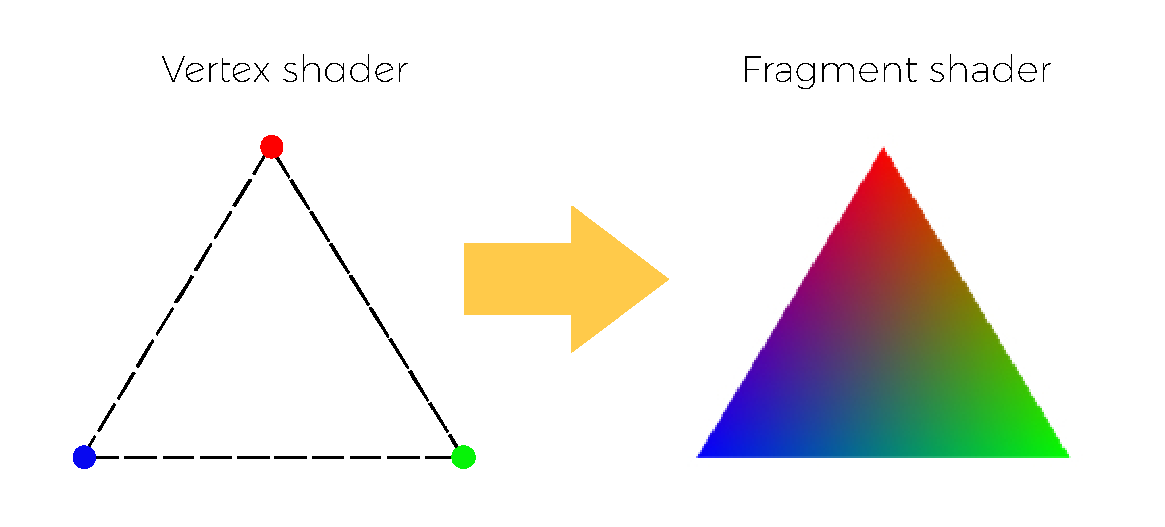
\includegraphics[scale=1.0,angle=0,width=1.0\linewidth]{obrazky-figures/interpolace}
	% 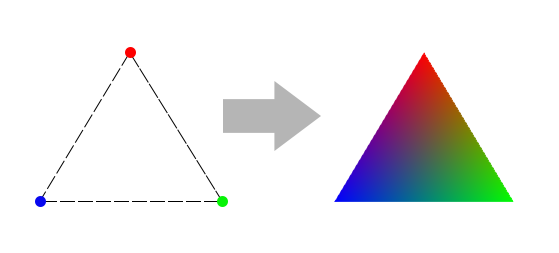
\includegraphics[scale=1.0,height=2.5in,angle=0]{obrazky-figures/interpolace.png}
	\caption{Ukázka interpolace hodnot mezi vertex a fragment shaderem.}
	\label{fig:inter}
\end{figure}
 



%=========================================================================
\newpage

\section{WebGL}
WebGL (\textbf{Web} \textbf{G}raphics \textbf{L}ibrary) je javascriptové aplikační rozhraní, které slouží pro nativní vykreslování 2D a 3D interaktivní grafiky přímo z webového prohlížeče \cite{mozilla}. K samotnému běhu WebGL není potřeba žádných dodatečných knihoven, nebo zásuvných modulů, protože je v tomto ohledu využívána přímo grafická karta. Program WebGL se v zásadě skládá z více jazyků, přičemž každý mů svůj vlastní účel a je nutné je používat dohromady. Jedním z nich je javascript, druhý je jazyk GLSL. V jazyce GLSL jsou napsány dva programy - vertex shader a fragment shader. Oba programy kompiluje ovladač grafické karty do kódu, který je poté vykonáván přímo na grafické kartě. Vertex shader i fragment shader mohou být předávány jako řetězce, takže manipulace s nimi je díky tomu značně zjednodušena. Velkou výhodou WebGL je integrace s DOM tudíž od automatické správy pamětí přes zpracování událostí až po jednoduché načítání bitmapy přímo v prostředí prohlížeče apod..

K samotnému vykreslení je použit již výše zmíněný element HTML5 \texttt{<canvas>}.

V současné době je oficiálně vydána verze WebGL 1.0, která je založeno na OpenGL ES 2.0. Doposud se jedná o jedinou stabilní verzi. OpenGL ES\footnote{OpenGL for Embedded Systems.} je zjednodušená verze OpenGL, která eliminuje většinu vykreslovacích pipeline. Tato verze je především určena pro menší vestavěné systémy. Dalším rozšířením WebGL bude verze 2.0, která se stále nachází ve vývoji. Bude založena na OpenGL ES 3.0 přinášející velká vylepšení v zobrazování 3D grafiky - zejména textur, akceleraci vizuálních efektů, novou verzí jazyka GLSL s plnou podporu desetinných a celočíselných operací apod.

\subsection{Vykreslování primitiv}
K vykreslení nějakého grafického prvku jsou potřeba v zásadě jen dvě věci - vrcholy přepočítané do tzv. \textit{clipspace} a jemu přiřazené odpovídající barvy. Jak pro vrcholy tak pro barvy slouží jiný GLSL shader. K vyobrazení objektu používá WebGL tří základní primitiva - vykreslení samotných bodů, čar nebo trojúhelníku. Vše funguje tak, že zadaný bod, kterému budeme chtít přiřadit barvu, se načte do odpovídající speciální globální proměnné ve vertex shaderu, tam se daná hodnota přepočítá do intervalu \texttt{<-1,1>} pro všechny jeho osy a vzniklá hodnota se uloží na grafické kartě. Počet bodu záleží na primitivu, které vykreslujeme. Pokud se tedy jedná o bod, stačí pouze jeden bod ve vertex shaderu, pokud se jedna o čáru tak dvě popř. trojúhelník, tak trojice bodů. GPU\footnote{Graphic Processing Unit - grafický procesor} poté zjistí, které pixely korespondují s vykreslovaným primitivem a pro každý takový pixel zavolá fragment shader. 


\subsection{Vyrovnávací paměť}
Buffery resp. vyrovnávací paměti jsou rychle přístupné paměti na grafické kartě. V bufferech jsou  uloženy potřebné data k vykreslování grafických objektů jako např. body geometrie, normály, mapování textur apod. Data jsou poté snadno dále předávány GLSL shaderům, které s nimi pracují.

%=========================================================================
\newpage

\subsection{Projekce}
Některé frameworky\footnote{Rámcová softwarová struktura usnadňující řešení dané problematiky} založené na WebGL zaměňují projekci za kameru, ta bohužel jako taková ve WebGL neexistuje. Jedná se pouze o způsob vykreslení grafické informace, ke které jsou využívány právě projekční zobrazení. WebGL podporuje dva základní typy projekce - ortografickou a perspektivní. 

Ortografická projekce využívá skutečné velikosti objektu. Scéna je reprezentována jako pravoúhlý hranol.

Perspektivní projekce zkresluje velikost objektů způsobem, jak je tomu v reálném světě. Čím je objekt dál od pozorovatele, tím se bude jevit jako menší, protože jeho pozice je středem této projekce. 
  
Pokud bychom chtěl vykreslit nejaký 3D objekt, bude potřeba mít v bufferech informace o vrcholech, normálách, textuře apod. Tyto data bychom zároveň museli neustále aktualizovat a nahrávat zpět do paměti, aby bylo možné s daným 3D objektem jakkoli manipulovat, posouvat apod. Aby nedocházelo k neustálému přepisování hodnot v paměti na GPU, veškeré změny zrealizujeme transformačními maticemi, kterými se bude geometrie objektu v paměti násobit, aniž by data v paměti byla jakkoli změněna.

\subsubsection{Homogenní souřadnice}
Homogenní souřadnice je tvořena čtyřmi prvky - \texttt{x}, \texttt{y}, \texttt{z} a \texttt{w}. První tři složky tvoří souřadnice euklidovského prostoru, poslední prvek \texttt{w} je perspektivní složka a spolu se souřadnicemi \texttt{x}, \texttt{y}, \texttt{z} tvoří projekční prostor.


\subsubsection{Model matrix}
Jedná se o matici, kterou držíme pro každý vykreslovaný objekt. Stará se o úpravu tvaru, natočení a posuvu objektu.

\subsubsection{View matrix}
Díky teto transformační matici realizujeme již avizovanou ``roli kamery'' , kdy simulujeme vzájemná vztah scény a pozorovatele.

\subsubsection{Perspective matrix}
Stará se o perspektivní zkreslení scény. Tato transformace rozhoduje o tom, jak velké zorné pole bude vykresleno a mapováno 
na obrazovku monitoru. 

%=========================================================================
\newpage

\subsection{Vytvoření a běh programu}
Po vytvoření kontextu \texttt{webgl} je již možné využívat funkce pro práci s WebGL. Funkce by se daly rozdělit na několik částí, nejprve ty, které pracují s shadery, dále ty které vytváří program, v neposlední řadě funkce pro prací s buffery a vykreslením dat. Všechny funkce WebGL pracují nad vytvořeným kontextem plátna\footnote{Vytvořený WebGL kontext budeme označovat jako \texttt{gl}}.

\begin{description}
	\item[\texttt{gl.createShader(type)}] - vytvoří objekt shaderu, vstupním argumenty \texttt{type} mohou být \\ \texttt{gl.VERTEX\_SHADER} nebo \texttt{gl.FRAGMENT\_SHADER}

	\item[\texttt{gl.shaderSource(shader, source)}] - asociuje objekt shaderu \texttt{shader} se zdrojovým kódem samotného shaderu \texttt{source} v textové formě
	
	\item[\texttt{gl.compileShader(shader)}] - kompiluje GLSL kód na binární data, vstupním parametrem je objekt shaderu \texttt{shader}

\end{description}

Následuje práce s programem. Funkce \texttt{gl.createProgram()} vytvoří objekt programu. Poté \texttt{gl.attachShader(program, shader)} - přiloží daný shader k programu.
Funkce \\ \texttt{gl.linkProgram(program)}, která slinkuje vše dohromady, \texttt{gl.useProgram(program)} - nastaví daný webgl program jako část současného vykreslovacího stavu.

\begin{description}
 
	\item[\texttt{gl.getAttribLocation(program, attribute)}] - vrací referenci na atribut v ve vertex shaderu

	\item[\texttt{gl.enableAttribute(attribute)}] - aktivuje atribut 
	
	\item[\texttt{gl.createBuffer()}] - vytvoří nový buffer objekt pro data
	
	\item[\texttt{gl.bindBuffer(target, buffer)}] - nastaví vytvořený buffer \texttt{buffer} jako aktivní, parametr \texttt{target} specifikuje data s jakými se bude pracovat

	\item[\texttt{gl.bufferData(target, srcData, usage)}] - parametr \texttt{target} má stejný význam jako u funkce \texttt{bindBuffer}, \texttt{srcData} určuje data, která se nahrají do bufferu, poslední parametr \texttt{usage} specifikuje způsob využiti uložených dat

	\item[\texttt{gl.vertexAttribPointer(attrib, size, type, normalized, stride, offset)}] -  \texttt{attrib} prováže atribut programu s aktivním bufferem, \texttt{size} určuje, z kolika prvků se skládají data v bufferu, \texttt{type} spcecifikuje datový typ dat v bufferu, \texttt{normalized} určuje zdali budou hodnoty normalizovány, parametr je typu \texttt{bool}, dále \texttt{stride} udávající zdali budeme nějaké hodnoty přeskakovat, \texttt{offset} odkud budeme data číst.


\end{description}

Samotné vykreslení uložených data v bufferech se realizuje funkcemi:


\begin{description}
	
	\item[\texttt{gl.drawArrays(mode, first, count)}] - vykresluje vstupní data. Parametr \texttt{mode} určuje, jaké grafické primitivum budem použito pro vykreslení, \texttt{first} určuje odkud se data zažnou upracovávat, \texttt{count} specifikuje počet vykreslovaných hodnot
	
	\item[\texttt{gl.drawElements(mode, count, type, offset)}] - stejně jako u \texttt{drawArrays()} určuje vykreslované grafické primitivum, to stejné se týká i parametru \texttt{count}, \texttt{type} definuje typ dat indexů a \texttt{offset} odkud začínáme zpracovávat indexy. HLavním rozdílem vůči funkci \texttt{drawArrays()} je ten, že \texttt{gl.drawElements(...)} nevykresluje body přímo, ale dostává jako vstupní data indexy na jednotlivé body, které vykresluje funkce \texttt{drawArrays()}
	
\end{description}

%=========================================================================
\newpage



\chapter{Návrh klíčových částí}
\label{chapter:3}
Kapitola nastiňuje, jakým způsobem jsou řešeny nejzásadnější problémy implementace prohlížeče. Snaží se navrhnout ty nejefektivnější způsoby řešení daných problémů a v případě, že tomu tak v konkrétním případě není, snaží se tyto  kroky návrhu jasně odůvodnit, proč jsou  daným způsobem takto řešeny.


\section{Geometrie}
Geometrie je potřebná k mapování textury, a to tak, aby daná textura reflektovala scénu co nejvěrněji. Kdybychom pro texturu nevytvářeli geometrii, na kterou se bude mapovat a jednoduše data namapovali do libovolné 2D roviny, dojde k významnému zkreslení pořizované scény.

K vyobrazení geometrie budeme využívat klasické pole, kde každý bod bude tvořen třemi rozměry v kartézské soustavě souřadnic, tedy formátu \texttt{[x1,y1,z1, x2,y2,z2, …]}, které utváří jednotlivé body v 3D prostoru. Body pak mezi sebou tvoří prostor, na který budou texturovací data  mapovaná. Ve WebGL umíme vykreslit jednotlivé body, čáry – tedy spojnice jednotlivých bodů, nebo trojúhelníky. V našem případě bude potřeba vykreslit texturu jako plochu, na kterou se bude vše mapovat. Pro ten to případ se ve WebGL používá vykreslení pomocí trojúhelníku, jako základní vykreslované primitivum plochy.

Geometrickým tělesem pro mapování bude zvolena koule, protože scéna resp. pořízená data, která budeme zpracovávat jsou zachycena ve sférickém modu a mapováním na kouli je dosažena nejvěrnější reprezentace scény.

Kouli so rozdělíme na poledníky a rovnoběžky. Poledníkem je v tomto případě myšlena spojnice severního a jižního pólu, kde úhel z počátku kartézské soustavy souřadnic mezi jednotlivými poledníky nabývá hodnot od 0 - 360\degree. Rovnoběžkou je myšlena kružnice  rovnoběžná se vzájemně sousedícími a svírající úhel s počátkem souřadnic od 0-180\degree. 

Je třeba tedy nejprve stanovit počet poledníků a rovnoběžek a z takových hodnot bude dále vypočítán úhel. Na základě úhlu budeme schopni přesně definovat bod v trojrozměrné rovině. Čím větší počet rovnoběžek a poledníků, tím bude geometrie věrněji aproximovat kouli - zvýší se hustota bodů v bufferech a tím bude i samotné vykreslení náročnější. Proto je ideální kompromis mezi jemností bodů a rychlosti načítání s téměř stejným výsledkem. Tato vlastnost by se nám hodila hlavně tedy v případech, kdy bychom měli vykreslit rozmanitý geometrický objekt se spoustou detailních sekvencí. V našem případě tento rozdíl tedy nepůjde okem rozeznat, takže skrze efektivitu je výhodné spíše snížit počet rovnoběžek a poledníků, čímž dosáhneme pozitivního efektu na samotnou rychlost programu.
\\\\
%Způsob vykreslení našich bodu určíme tedy řádkem: gl.drawElements(gl.TRINAGLES, 6, gl.UNSIGNED\_BYTE, 0), kde tedy říkáme že chceme vykreslovat plochu pomocí trojúhelníků, víz výše. (gl.TRINAGLES), druhým parametrem říkáme, kolik hodnot z index bufferu budeme potřebovat vykreslit, třetím parametrem oznamujeme velikost jednoho indexu a posledním parametrem říkáme, odkud začíná program číst naše body. Mohli bychom naše body vykreslovat ve webgl i pomoci příkazu: gl.drawArrays(), ale došlo by pak k situaci, že by se nám již vykreslené body zbytečně vykreslovali znovu. Abychom předešli duplikaci při vykreslování, bude nutné si vytvořit pole indexů, které nám budou ukazovat na jednotlivé vrcholy geometrie. Zde se již mohou indexy opakovat.%

\subsection{Sférický souřadný systém}

Každá rovnoběžka má po svém obvodu průsečíky s jednotlivými poledníky, tyto průsečíky jsou naše body geometrie, které budou nahrány do bufferů. Jelikož každá rovnoběžka nabývá úhlu od 0 do 180\degree  resp. $0-\pi$, tak tento úhel můžeme podělit počtem rovnoběžek a vynásobit aktuální rovnoběžkou, čímž získáme svíraný úhel s počátkem souřadnic. Na obrázku \ref{fig:geom} označujeme tento úhel jako $\theta$. Provedením této operaci pro všechny horizontální obvodové kružnice, vypočítáme všechny svírané úhly s počátkem souřadnic. 

Dále je nutné vypočítat svíraný úhel všech poledníků - vertikálních čar svírajících jej s počátkem souřadnic. Na obrázku \ref{fig:geom} je vyznačen jako $\varphi$. Jak jsem již nastínil výše, $\varphi$ nabývá hodnot od 0 do 360\degree resp. $0-2\pi$. Vytyčený úhel mezi jednotlivými čarami jsme schopni spočítat tak, že jej podělíme počtem vertikálních čar a vynásobíme aktuálním poledníkem. Takto získáme rovnoměrné rozložení bodů na celé rovnoběžce. Provedením  operace pro všechny rovnoběžky již bude geometrie koule z hlediska úhlů kompletní.

\begin{figure}[h]
	\label{img:2}
	\centering
	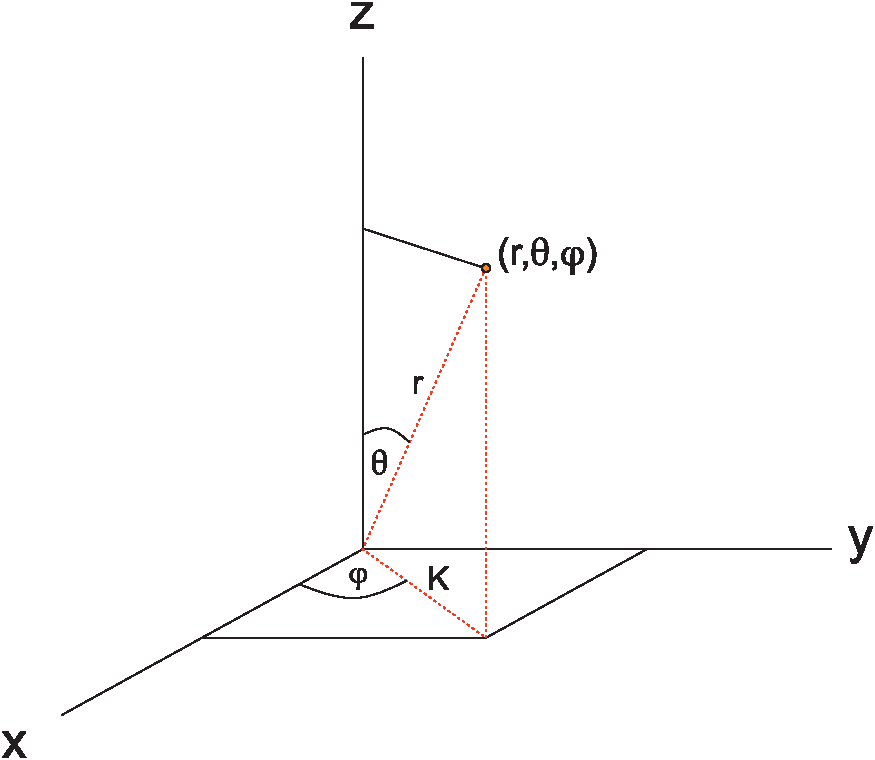
\includegraphics[scale=1.0,angle=0,width=0.8\linewidth]{obrazky-figures/geometry}
	\caption{Výpočet jednotlivých bodů geometrie}
	\label{fig:geom}
\end{figure}
 
Na základě vypočtených úhlů, je možné již spočítat jednotlivé složky kartézské soustavy souřadnic \texttt{[x,y,z]} každému bodu, čímž dojde ke kompletní aproximaci tělesa.

%=========================================================================
\newpage

K výpočtu využijeme goniometrické funkce  a vztahy v pravoúhlém trojúhelníku. Jelikož $ \cos (\varphi) $ je dána poměrem délky přilehlé odvěsny a přeponou \cite{Goniometrie}, tak souřadnici \texttt{\textit{x}} definujeme vtahem:
 
\begin{equation}
 \cos (\varphi) = \frac{x}{K}  \Rightarrow x = \cos (\varphi) \cdot K
\end{equation}
\\
Ze vzniklého vztahu jasně vidíme, že je třeba dopočítat přeponu \textit{K} v trojúhelníku  o stranách $\arrowvert xKy\arrowvert$, kterou ale odvodíme vztahem odvěsny \textit{K} v trojúhelníku $\arrowvert zrK\arrowvert$. Mezi odvěsnou \texttt{K}\footnote{Z obrázku \ref{fig:geom} je patrné, že je přeponou v $\bigtriangleup$ $\arrowvert xKy\arrowvert$, ale odvěsnou v $\bigtriangleup$ $\arrowvert zrK\arrowvert$} a protilehlou přeponou \textit{r} platí, že délka odvěsny protilehlé k úhlu $\varphi$ a délka přepony \cite{Goniometrie} mají vztah:
\\
\begin{equation}
\label{math:K}
\sin (\theta) = \frac{K}{r}  \Rightarrow K = \sin (\theta) \cdot r
\end{equation}
\\
Všechny neznáme máme již dopočítané a můžeme dosadit do první rovnice, čímž dostáváme výsledný vztah převedené souřadnice z kartézské soustavy souřadnic do sférického souřadného systému:
\\
\begin{equation}
\label{math:x}
x = \sin (\theta) \cdot  \cos (\varphi) \cdot r
\end{equation}
\\
Následující souřadnici \texttt{y} vyjádříme obdobným vztahem jako u předchozí souřadnice, ale s tím rozdílem, že protilehlá odvěsna bude k úhlu $\varphi$ a přeponou bude strana \texttt{K}:
\\
\begin{displaymath}
\sin (\varphi) = \frac{y}{K}  \Rightarrow y = \sin (\varphi) \cdot K
\end{displaymath}
\\
Opět máme v rovnici pro výpočet souřadnice \texttt{y} stranu \texttt{K}, kterou ale máme již vypočtenou ve vztahu \ref{math:K}, tudíž už jen tento vztah dosadíme a vznikne výsledná rovnice hledané  souřadnice:
\\
\begin{equation}
\label{math:y}
y = \sin (\varphi) \cdot \sin (\theta) \cdot r
\end{equation}
\\
Poslední souřadnice \texttt{z} je značně jednodušší, protože nám odpadá proměnná \texttt{K}. Vyjádření souřadnice \texttt{z} je principiálně úplně stejné, jako tomu bylo u souřadnice \texttt{x} - přilehlá odvěsna k úhlu $\varphi$ ku přeponě \texttt{r}. Výsledný vztah je tedy možné vyjádřit následovně:
\\
\begin{equation}
\label{math:z}
\cos (\varphi) = \frac{z}{r} \Rightarrow z = \cos (\varphi) \cdot r
\end{equation}

%=========================================================================
\newpage


\subsection{Vrcholy}
Jakmile máme vypočítány konkrétní složky trojrozměrného prostoru, můžeme přistoupit ke kompletaci dat určených k nahrání do grafické karty. Těmito daty jsou vrcholy samotné geometrie, texturovací data a indexy. 

Získání samotného vrcholu lze vynásobením složek \texttt{x}, \texttt{y} a \texttt{z} průměrem tělesa \texttt{r}. Tato operace musí být provedena u všech bodů koule.

Vzniklé těleso vyobrazené pomocí čar\footnote{Použito grafické primitivum \texttt{gl.LINES}.} je demonstrováno na obr. \ref{img:3}.


\begin{figure}[h]
	\label{img:3}
	\centering
	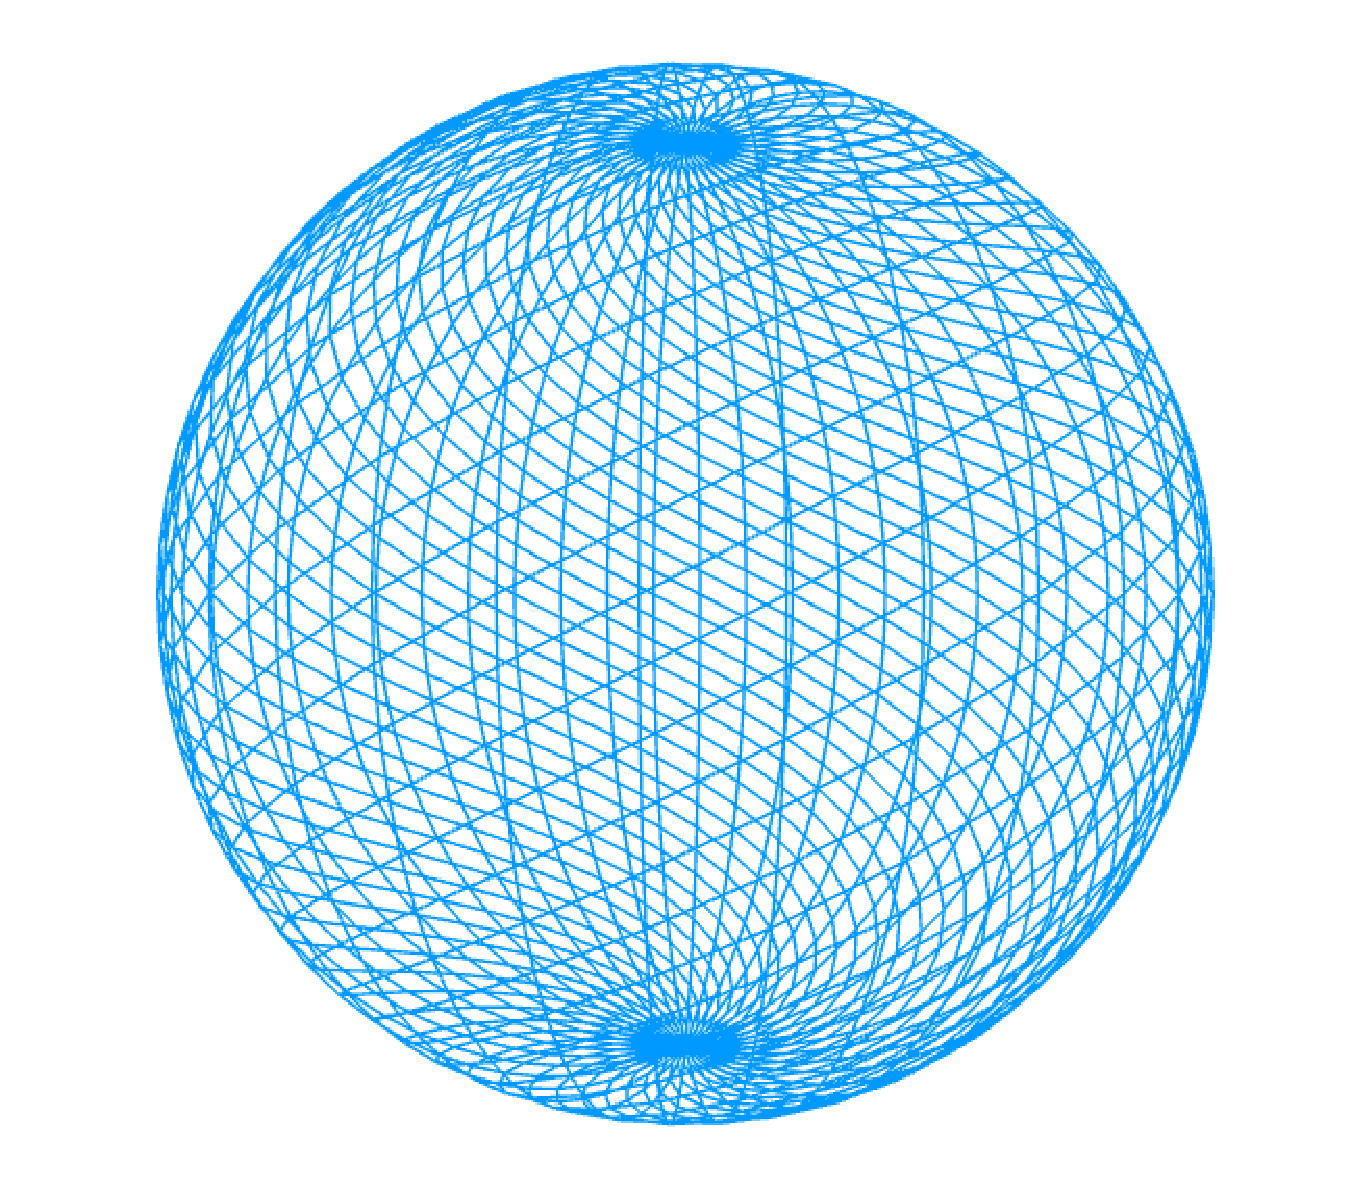
\includegraphics[scale=1.0,angle=0,width=0.7\linewidth]{obrazky-figures/vertex}
	\caption{Koule vyobrazena pomocí čar}
	\label{fig:geom2}
\end{figure}


\subsection{Textura}
\subsection{indexy}





\section{Korekce textur}


\cite{geometrie}
 


\section{Projekce}
\subsection{Modelová matice}
\subsection{Zobrazovací matice}
\subsection{Perspektivní matice}

\section{Metadata}

%=========================================================================
\newpage

\section{Zorný úhel}
Zorný úhel je grafický prvek, který udává informace o aktuálním zorném poli zobrazovací matice. Tento úhel se mění na základě přibližování, nebi oddalování scény od pozorovatele. 

\subsection{Návrh prvku}
K vyobrazení prvku budeme potřebovat vektor svg zobrazující přímý úhel. Reprezentován bude tvarem polokoule, u které se využije vlastnosti tahu. Ve vektorové grafice se jedná o nastavení atributu \texttt{stroke-width}, který bude reprezentovat zorný úhel. Důvodem, přoč pro vyobrazení samotné není využita samotná křivka vyplněná barvou je ten, že pokud se přenastaví úhel zobrazení, tak se křivka zdeformuje tak, že z ní není zjevný zorný úhel.

Vstupními argumenty je pozice prvku pomoci ve dvojrozměrném prostoru \texttt{(x,y)} a průměr kruhu. Dále je potřeba přepočítat tyto souřadnice dvojrozměrného prostoru na sférické souřadnice. K samotnému výpočtu dostačuje Pythagorova věta, kdy pomocí bodu (x,y) jsou známy hodnoty odvěsen a je možní spočítat přeponu. Takto odvodíme vztahy pro \texttt{x} a \texttt{y}

\begin{description}
	\item [{\LARGE $ x = r\cdot\cos(\theta) $}] 
	\item [{\LARGE $ y = r\cdot\sin(\theta) $}]
\end{description}
 


%=========================================================================
\newpage


\section{Kompas}

\section{Blending}
%=========================================================================

\chapter{Implementace panoramatického prohlížeče}
\label{chapter:4}


\section{Grafické rozhraní}
Veškeré prvky, které nejsou vykreslovány skrze grafickou kartu, se v elementu jak již bylo nastíněno v předcházejících kapitolách, \texttt{<canvas>} nezobrazí z důvodu, že je vše skryto. Jen v případě, že by prohlížeč nepodporoval plátno, zobrazí co je v něm. Realizaci samotných prvků jako je kompas, nebo zorný úhel až po ovládací prvky videa, bude třeba realizovat za pomocí kaskádových stylů, kdy pomocí dynamického pozicování budeme všechny prvky zobrazovat překryvem plátna.

\section{Kompas}
Prvek překrývající plátno \texttt{<canvas>}. Vstupnímí metadaty jsou zadány koordinační body severu, popř. jihu. Díky interakcí s myší - tedy násobení zobrazovací transformační maticí realizujeme pohyb pozorovatele, čímž se mění prostorové úhel, který ovlivňuje odchylku severu, popř. jihu od původní zadané pozice v metadatech.

Samotná konstrukce kompasu je zasazena do tagu \texttt{<div id="compass-box">}. Funkce, která nahraje data do kontejneru kompasu se nazývá \texttt{createCompass()}.

\subsection{Pozicování}
Vytvoření samotného kompasu realizuje funkce \texttt{createCompass(width, height)}, argument \texttt{width} udává šířku kompasu, argument \texttt{height} zase jeho výšku. Pozice kompasu v plátně je realizována pomocí nastavení hodnot \texttt{div.style.left} a 
\texttt{div.style.top} v pixelech, kde se bude udávat výsledná hodnota posuvu. Pozici samotnou nastavuje řádek \texttt{div.style.position = 'absolute';}. Posun  od levého okraje obrazovky \texttt{div.style.left} je vypočten tak, že si načteme celkovou šířku

%=========================================================================
\newpage

\section{Zorný úhel}


Pravidla \cite{Kompendium}. Pravidla \cite{Goniometrie}. 
Goniometrie
\chapter{Testování}
\label{chapter:5}


\chapter{Závěr}
\label{chapter:6}

Závěrečná kapitola obsahuje zhodnocení dosažených výsledků se zvlášť vyznačeným vlastním přínosem studenta. Povinně se zde objeví i zhodnocení z pohledu dalšího vývoje projektu, student uvede náměty vycházející ze zkušeností s řešeným projektem a uvede rovněž návaznosti na právě dokončené projekty.

%=========================================================================
 % viz. obsah.tex / see obsah.tex

  % Pouzita literatura / Bibliography
  % ----------------------------------------------
\ifslovak
  \makeatletter
  \def\@openbib@code{\addcontentsline{toc}{chapter}{Literatúra}}
  \makeatother
  \bibliographystyle{bib-styles/czechiso}
\else
  \ifczech
    \makeatletter
    \def\@openbib@code{\addcontentsline{toc}{chapter}{Literatura}}
    \makeatother
    \bibliographystyle{bib-styles/czechiso}
  \else 
    \makeatletter
    \def\@openbib@code{\addcontentsline{toc}{chapter}{Bibliography}}
    \makeatother
    \bibliographystyle{bib-styles/englishiso}
  %  \bibliographystyle{alpha}
  \fi
\fi
  \begin{flushleft}
  \bibliography{projekt-20-literatura-bibliography}
  \end{flushleft}

  % vynechani stranky v oboustrannem rezimu
  % Skip the page in the two-sided mode
  \iftwoside
    \cleardoublepage
  \fi

  % Prilohy / Appendices
  % ---------------------------------------------
  \appendix
\ifczech
  \renewcommand{\appendixpagename}{Přílohy}
  \renewcommand{\appendixtocname}{Přílohy}
  \renewcommand{\appendixname}{Příloha}
\fi
\ifslovak
  \renewcommand{\appendixpagename}{Prílohy}
  \renewcommand{\appendixtocname}{Prílohy}
  \renewcommand{\appendixname}{Príloha}
\fi
  \appendixpage

% vynechani stranky v oboustrannem rezimu
% Skip the page in the two-sided mode
\iftwoside
  \cleardoublepage
\fi
  
\ifslovak
%  \section*{Zoznam príloh}
%  \addcontentsline{toc}{section}{Zoznam príloh}
\else
  \ifczech
%    \section*{Seznam příloh}
%    \addcontentsline{toc}{section}{Seznam příloh}
  \else
%    \section*{List of Appendices}
%    \addcontentsline{toc}{section}{List of Appendices}
  \fi
\fi
  \startcontents[chapters]
  % seznam příloh / list of appendices
  \section*{Seznam příloh}
     \printcontents[chapters]{l}{0}{\setcounter{tocdepth}{2}}
  
  % vynechani stranky v oboustrannem rezimu
  \iftwoside
    \cleardoublepage
  \fi
  % Tento soubor nahraďte vlastním souborem s přílohami (nadpisy níže jsou pouze pro příklad)
% This file should be replaced with your file with an appendices (headings below are examples only)

% Umístění obsahu paměťového média do příloh je vhodné konzultovat s vedoucím
% Placing of table of contents of the memory media here should be consulted with a supervisor
%\chapter{Obsah přiloženého paměťového média}

%\chapter{Manuál}

%\chapter{Konfigurační soubor} % Configuration file

%\chapter{RelaxNG Schéma konfiguračního souboru} % Scheme of RelaxNG configuration file

%\chapter{Plakát} % poster

\chapter{Jak pracovat s touto šablonou}
\label{jak}

V této kapitole je uveden popis jednotlivých částí šablony, po kterém následuje stručný návod, jak s touto šablonou pracovat. 

Jedná se o přechodnou verzi šablony. Nová verze bude zveřejněna do konce roku 2016 a bude navíc obsahovat nové pokyny ke správnému využití šablony, závazné pokyny k~vypracování bakalářských a diplomových prací (rekapitulace pokynů, které jsou dostupné na~webu) a nezávazná doporučení od vybraných vedoucích. Jediné soubory, které se v nové verzi změní, budou projekt-01-kapitoly-chapters.tex a projekt-30-prilohy-appendices.tex, jejichž obsah každý student vymaže a nahradí vlastním. Šablonu lze tedy bez problémů využít i~v~současné verzi.

\section*{Popis částí šablony}

Po rozbalení šablony naleznete následující soubory a adresáře:
\begin{DESCRIPTION}
  \item [bib-styles] Styly literatury (viz níže). 
  \item [obrazky-figures] Adresář pro Vaše obrázky. Nyní obsahuje placeholder.pdf (tzv. TODO obrázek, který lze použít jako pomůcku při tvorbě technické zprávy), který se s prací neodevzdává. Název adresáře je vhodné zkrátit, aby byl jen ve zvoleném jazyce.
  \item [template-fig] Obrázky šablony (znak VUT).
  \item [fitthesis.cls] Šablona (definice vzhledu).
  \item [Makefile] Makefile pro překlad, počítání normostran, sbalení apod. (viz níže).
  \item [projekt-01-kapitoly-chapters.tex] Soubor pro Váš text (obsah nahraďte).
  \item [projekt-20-literatura-bibliography.bib] Seznam literatury (viz níže).
  \item [projekt-30-prilohy-appendices.tex] Soubor pro přílohy (obsah nahraďte).
  \item [projekt.tex] Hlavní soubor práce -- definice formálních částí.
\end{DESCRIPTION}

Výchozí styl literatury (czechiso) je od Ing. Martínka, přičemž anglická verze (englishiso) je jeho překladem s drobnými modifikacemi. Oproti normě jsou v něm určité odlišnosti, ale na FIT je dlouhodobě akceptován. Alternativně můžete využít styl od Ing. Radima Loskota nebo od Ing. Radka Pyšného\footnote{BP Ing. Radka Pyšného \url{http://www.fit.vutbr.cz/study/DP/BP.php?id=7848}}. Alternativní styly obsahují určitá vylepšení, ale zatím nebyly řádně otestovány větším množstvím uživatelů. Lze je považovat za beta verze pro zájemce, kteří svoji práci chtějí mít dokonalou do detailů a neváhají si nastudovat detaily správného formátování citací, aby si mohli ověřit, že je vysázený výsledek v pořádku.

Makefile kromě překladu do PDF nabízí i další funkce:
\begin{itemize}
  \item přejmenování souborů (viz níže),
  \item počítání normostran,
  \item spuštění vlny pro doplnění nezlomitelných mezer,
  \item sbalení výsledku pro odeslání vedoucímu ke kontrole (zkontrolujte, zda sbalí všechny Vámi přidané soubory, a případně doplňte).
\end{itemize}

Nezapomeňte, že vlna neřeší všechny nezlomitelné mezery. Vždy je třeba manuální kontrola, zda na konci řádku nezůstalo něco nevhodného -- viz Internetová jazyková příručka\footnote{Internetová jazyková příručka \url{http://prirucka.ujc.cas.cz/?id=880}}.

\paragraph {Pozor na číslování stránek!} Pokud má obsah 2 strany a na 2. jsou jen \uv{Přílohy} a~\uv{Seznam příloh} (ale žádná příloha tam není), z nějakého důvodu se posune číslování stránek o 1 (obsah \uv{nesedí}). Stejný efekt má, když je na 2. či 3. stránce obsahu jen \uv{Literatura} a~je možné, že tohoto problému lze dosáhnout i jinak. Řešení je několik (od~úpravy obsahu, přes nastavení počítadla až po sofistikovanější metody). \textbf{Před odevzdáním proto vždy překontrolujte číslování stran!}


\section*{Doporučený postup práce se šablonou}

\begin{enumerate}
  \item \textbf{Zkontrolujte, zda máte aktuální verzi šablony.} Máte-li šablonu z předchozího roku, na stránkách fakulty již může být novější verze šablony s~aktualizovanými informacemi, opravenými chybami apod.
  \item \textbf{Zvolte si jazyk}, ve kterém budete psát svoji technickou zprávu (česky, slovensky nebo anglicky) a svoji volbu konzultujte s vedoucím práce (nebyla-li dohodnuta předem). Pokud Vámi zvoleným jazykem technické zprávy není čeština, nastavte příslušný parametr šablony v souboru projekt.tex (např.: \verb|documentclass[english]{fitthesis}| a přeložte prohlášení a poděkování do~angličtiny či slovenštiny.
  \item \textbf{Přejmenujte soubory.} Po rozbalení je v šabloně soubor projekt.tex. Pokud jej přeložíte, vznikne PDF s technickou zprávou pojmenované projekt.pdf. Když vedoucímu více studentů pošle projekt.pdf ke kontrole, musí je pracně přejmenovávat. Proto je vždy vhodné tento soubor přejmenovat tak, aby obsahoval Váš login a (případně zkrácené) téma práce. Vyhněte se však použití mezer, diakritiky a speciálních znaků. Vhodný název tedy může být např.: \uv{xlogin00-Cisteni-a-extrakce-textu.tex}. K přejmenování můžete využít i přiložený Makefile:
\begin{verbatim}
make rename NAME=xlogin00-Cisteni-a-extrakce-textu
\end{verbatim}
  \item Vyplňte požadované položky v souboru, který byl původně pojmenován projekt.tex, tedy typ, rok (odevzdání), název práce, svoje jméno, ústav (dle zadání), tituly a~jméno vedoucího, abstrakt, klíčová slova a další formální náležitosti.
  \item Nahraďte obsah souborů s kapitolami práce, literaturou a přílohami obsahem svojí technické zprávy. Jednotlivé přílohy či kapitoly práce může být výhodné uložit do~samostatných souborů -- rozhodnete-li se pro toto řešení, je doporučeno zachovat konvenci pro názvy souborů, přičemž za číslem bude následovat název kapitoly. 
  \item Nepotřebujete-li přílohy, zakomentujte příslušnou část v projekt.tex a příslušný soubor vyprázdněte či smažte. Nesnažte se prosím vymyslet nějakou neúčelnou přílohu jen proto, aby daný soubor bylo čím naplnit. Vhodnou přílohou může být obsah přiloženého paměťového média.
  \item Nascanované zadání uložte do souboru zadani.pdf a povolte jeho vložení do práce parametrem šablony v projekt.tex (\verb|documentclass[zadani]{fitthesis}|).
  \item Nechcete-li odkazy tisknout barevně (tedy červený obsah -- bez konzultace s vedoucím nedoporučuji), budete pro tisk vytvářet druhé PDF s tím, že nastavíte parametr šablony pro tisk: (\verb|documentclass[zadani,print]{fitthesis}|).  Barevné logo se nesmí tisknout černobíle!
  \item Vzor desek, do kterých bude práce vyvázána, si vygenerujte v informačním systému fakulty u zadání. Pro disertační práci lze zapnout parametrem v šabloně (více naleznete v souboru fitthesis.cls).
  \item Nezapomeňte, že zdrojové soubory i (obě verze) PDF musíte odevzdat na CD či jiném médiu přiloženém k technické zprávě.
\end{enumerate}

\subsection*{Pokyny pro oboustranný tisk}
\begin{itemize}
\item Zapíná se parametrem šablony: \verb|\documentclass[twoside]{fitthesis}|
\item Po vytištění oboustranného listu zkontrolujte, zda je při prosvícení sazební obrazec na obou stranách na stejné pozici. Méně kvalitní tiskárny s duplexní jednotkou mají často posun o 1--3 mm. Toto může být u některých tiskáren řešitelné tak, že vytisknete nejprve liché stránky, pak je dáte do stejného zásobníku a vytisknete sudé.
\item Za titulním listem, obsahem, literaturou, úvodním listem příloh, seznamem příloh a případnými dalšími seznamy je třeba nechat volnou stránku, aby následující část začínala na liché stránce (\textbackslash cleardoublepage).
\item  Konečný výsledek je nutné pečlivě překontrolovat.
\end{itemize}


\subsection*{Užitečné nástroje}
\label{nastroje}

Následující seznam není výčtem všech využitelných nástrojů. Máte-li vyzkoušený osvědčený nástroj, neváhejte jej využít. Pokud však nevíte, který nástroj si zvolit, můžete zvážit některý z následujících:

\begin{description}
	\item[\href{http://miktex.org/download}{MikTeX}] \LaTeX{} pro Windows -- distribuce s jednoduchou instalací a vynikající automatizací stahování balíčků.
	\item[\href{http://texstudio.sourceforge.net/}{TeXstudio}] Přenositelné opensource GUI pro \LaTeX{}.  Ctrl+klik umožňuje přepínat mezi zdrojovým textem a PDF. Má integrovanou kontrolu pravopisu, zvýraznění syntaxe apod. Pro jeho využití je nejprve potřeba nainstalovat MikTeX.
	\item[\href{http://jabref.sourceforge.net/download.php}{JabRef}] Pěkný a jednoduchý program v Javě pro správu souborů s bibliografií (literaturou). Není potřeba se nic učit -- poskytuje jednoduché okno a formulář pro editaci položek.
	\item[\href{https://inkscape.org/en/download/}{InkScape}] Přenositelný opensource editor vektorové grafiky (SVG i PDF). Vynikající nástroj pro tvorbu obrázků do odborného textu. Jeho ovládnutí je obtížnější, ale výsledky stojí za to.
	\item[\href{https://git-scm.com/}{GIT}] Vynikající pro týmovou spolupráci na projektech, ale může výrazně pomoci i jednomu autorovi. Umožňuje jednoduché verzování, zálohování a přenášení mezi více počítači.
	\item[\href{http://www.overleaf.com/}{Overleaf}] Online nástroj pro \LaTeX{}. Přímo zobrazuje náhled a umožňuje jednoduchou spolupráci (vedoucí může průběžně sledovat psaní práce), vyhledávání ve zdrojovém textu kliknutím do PDF, kontrolu pravopisu apod. Zdarma jej však lze využít pouze s určitými omezeními (někomu stačí na disertaci, jiný na ně může narazit i při psaní bakalářské práce) a pro dlouhé texty je pomalejší.
\end{description}

\subsection*{Užitečné balíčky pro \LaTeX}

Studenti při sazbě textu často řeší stejné problémy. Některé z nich lze vyřešit následujícími balíčky pro \LaTeX:

\begin{itemize}
  \item \verb|amsmath| -- rozšířené možnosti sazby rovnic,
  \item \verb|float, afterpage, placeins| -- úprava umístění obrázků,
  \item \verb|fancyvrb, alltt| -- úpravy vlastností prostředí Verbatim, 
  \item \verb|makecell| -- rozšíření možností tabulek,
  \item \verb|pdflscape, rotating| -- natočení stránky o 90 stupňů (pro obrázek či tabulku),
  \item \verb|hyphenat| -- úpravy dělení slov,
  \item \verb|picture, epic, eepic| -- přímé kreslení obrázků.
\end{itemize}

Některé balíčky jsou využity přímo v šabloně (v dolní části souboru fitthesis.cls). Nahlédnutí do jejich dokumentace může být rovněž užitečné.

Sloupec tabulky zarovnaný vlevo s pevnou šířkou je v šabloně definovaný \uv{L} (používá se jako \uv{p}).

 % viz. prilohy.tex / see prilohy.tex
\end{document}
